\subsection{Gépi tanulás}
\begin{frame}{Gépi tanulás}
    \begin{itemize}
        \item Egy algoritmus tanul, ha egy feladat megoldása során olyan változások következnek be a működésében, hogy később ugyanazt a feladatot jobban (eredmény, hatékonyság) képes megoldani, mint korábban
        \item Konkrét utasítások nélkül
        \item Matematikai modell készítése
        \item Felügyelt, felügyelet nélküli, megerősítéses tanulás
    \end{itemize}
\end{frame}

\begin{frame}{Felügyelt tanulás}
    \begin{itemize}
        \item {\bf Tanító minta}: a minták elvárt kimenete ismert
        % \item {\bf Tanító minta} input-output párokkal: $(x_1, y_1), (x_2, y_2), \dots (x_N, y_N)$
        %     \begin{itemize}
        %         \item Minden $y_j$ valami $y = f(x)$ ismeretlen függvényre illeszkedik
        %         \item Keresünk egy $h$ függvényt, ami a lehető legpontosabban közelíti $f$-t
        %     \end{itemize}
        \item {\bf Teszt mintával} ellenőrizzük az illesztés pontosságát
        % \item Műkedvelőknek: $$\min \frac{1}{N} \sum_{n=1}^{N} \mathcal{L}(f(\Theta, x_n), y_n)$$
        \item Két nagy csoport: osztályozás és regresszió (előrejelzés)
        \item Példák: időjárás-előrejelzés, népességnövekedés, kép és spam felismerése (Feladat: melyik példa melyik csoportba tartozik?)
        \item Ez akkor működik, ha
        \begin{itemize}
            \item Elég nagy mintánk van (drága összegyűjteni)
            \item $f$-et jól választjuk meg
        \end{itemize}
    \end{itemize}
    
    % \centering\includegraphics[scale=0.4]{figures/knn-classification.png}
    % \includegraphics[scale=0.2]{figures/knn-regression.png}
\end{frame}

\begin{frame}{Felügyelt tanulás}
    \centering
    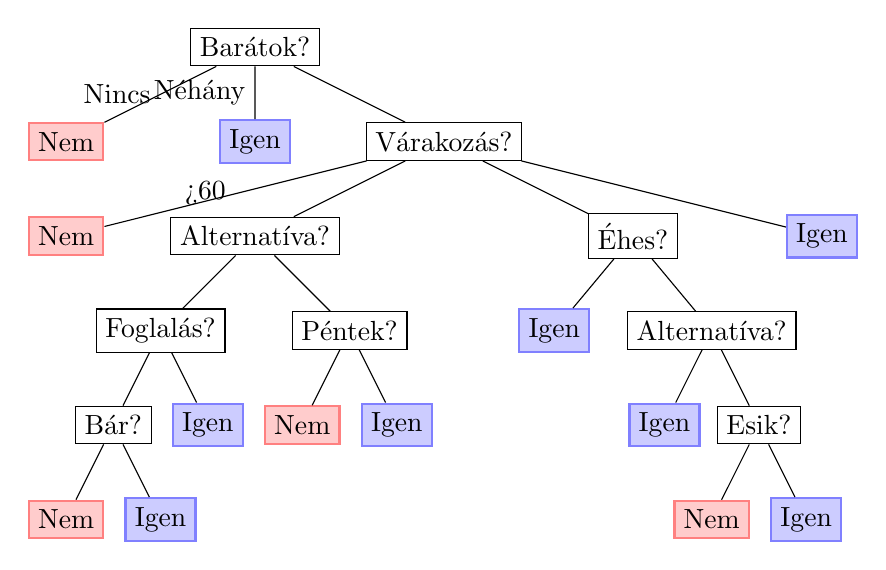
\begin{tikzpicture}
        [
        scale=0.8,
         % Styles
         no/.style={rectangle,draw=red!50,fill=red!20,thick},
         yes/.style={rectangle,draw=blue!50,fill=blue!20,thick},
         q/.style={rectangle,draw}
        ] 
        %  level distance=4mm,
        %  level 1/.style={sibling distance=20mm},
        %  level 2/.style={sibling distance=30mm},
        %  level 3/.style={sibling distance=35mm},
        %  level 4/.style={sibling distance=40mm},
        %  level 5/.style={sibling distance=45mm}
        

        \node[q] (root) {Barátok?}
            [sibling distance=30mm]
            child { node[no] {Nem} 
                edge from parent
                    node[left] {Nincs}
            }
            child { node[yes] {Igen} 
                edge from parent
                    node[left] {Néhány}
            }
            child { node[q] {Várakozás?}
                % edge from parent node[right] {Sok}
                [sibling distance=30mm]
                child { node[no] {Nem} 
                    edge from parent
                        node[left] {>60}
                }
                child { node[q] {Alternatíva?}
                    [sibling distance=30mm]
                    child { node[q] {Foglalás?} 
                        [sibling distance=15mm]
                        child { node[q] {Bár?}
                            child { node[no] {Nem} }
                            child { node[yes] {Igen} } 
                            }
                        child { node[yes] {Igen} } 
                        }
                    child { node[q] {Péntek?}
                        [sibling distance=15mm]
                        child { node[no] {Nem} }
                        child { node[yes] {Igen} } 
                        } 
                    }
                child[missing] { node[y] {Igen} }
                child { node[q] {Éhes?}
                    [sibling distance=25mm]
                    child { node[yes] {Igen} }
                    child { node[q] {Alternatíva?}
                        [sibling distance=15mm]
                        child { node[yes] {Igen} }
                        child { node[q] {Esik?} 
                        [sibling distance=15mm]
                            child { node[no] {Nem} }
                            child { node[yes] {Igen} }
                            }
                        }
                    }
                child { node[yes] {Igen} } };
    \end{tikzpicture}
    % \begin{tikzpicture}
    %     [scale=0.1,
    %      % Styles
    %      no/.style={rectangle,draw=red!50,fill=red!20,thick},
    %      yes/.style={rectangle,draw=blue!50,fill=blue!20,thick},
    %      question/.style={rectangle,draw}]

    %     \node[no] (n1) {Nem};
    %     \node[yes] (y1) [right=of n1] {Igen};
    %     \node[question] (q1) [above=of y1] {Barátok?}
    %         edge [->] (n1)
    %         edge [->] (y1);
        
    %     \node[no] (n2) [below=of y1] {Nem};
    %     \node[question] (q2) [right=of y1] {Várakozási idő?}
    %         edge [<-] (q1)
    %         edge [->] (n2);
    %     \node[question] (q3) [right=of n2] {Alternatív?}
    %         edge [<-] (q2);
    %     \node[question] (q4) [right=of q3] {Éhes?}
    %         edge [<-] (q2);
    %     \node[yes] (y2) [right=of q4] {Igen}
    %         edge [<-] (q2);
            
    %     \node[question] (q5) [below left=of q3] {Foglalás?}
    %         edge [<-] (q3);
    %     \node[question] (q6) [below right=of q3] {P/Szo?}
    %         edge [<-] (q3);
        
    %     \node[question] (q7) [below left=of q5] {Bár?}
    %         edge [<-] (q5);
    %     \node[yes] (q8) [right=of q7] {Igen}
    %         edge [<-] (q5);
    %     \node[no] (n3) [below left=of q7] {Nem}
    %         edge [<-] (q7);
    %     \node[yes] (y4) [below right=of q7] {Igen}
    %         edge [<-] (q7);
        
    % \end{tikzpicture}
\end{frame}


\begin{frame}{Nemfelügyelt tanulás}
    \begin{itemize}
        \item Tanító minta csak input adatokkal - nem ismert, hogy az adat micsoda
        \item Úgy csoportosítunk, hogy a hasonlók egy csoportba kerüljenek
    \end{itemize}
    
    \centering
    \begin{tikzpicture}
        \node<1> (img1) {\includegraphics[scale=0.25]{figures/k-means-1.png}};
        \node<2> (img2) {\includegraphics[scale=0.25]{figures/k-means-2.png}};
        \node<3> (img3) {\includegraphics[scale=0.25]{figures/k-means-3.png}};
        \node<4> (img4) {\includegraphics[scale=0.25]{figures/k-means-4.png}};
        \node<5> (img5) {\includegraphics[scale=0.25]{figures/k-means-5.png}};
        \node<6> (img6) {\includegraphics[scale=0.25]{figures/k-means-6.png}};
        
        % \node<7> (img7) {\includegraphics[scale=0.6]{figures/color1.png}};
        % \node<8> (img8) {\includegraphics[scale=0.6]{figures/color2.png}};
        % \node<9> (img9) {\includegraphics[scale=0.6]{figures/color3.png}};
    \end{tikzpicture}
\end{frame}

\begin{frame}{Megerősítéses tanulás}
    \begin{itemize}
        % \item Példa: \href{https://deepmind.com/research/case-studies/alphago-the-story-so-far}{AlphaGo} (2015 október, 5-0)
        \item Példa:
        \begin{itemize}
            \item \href{https://www.youtube.com/watch?v=VMp6pq6_QjI}{AI Learns to Park (Youtube)}
            \item \href{https://www.youtube.com/watch?v=CqYKhbyHFtA}{Two AI Fight for the same parking spot (Youtube)}
        \end{itemize}
        \item Nincs visszajelzés, hogy mi a jó vagy rossz
        \item Az algoritmus {\it megtanulja}, hogy melyik a jó lépés
        \item Mi lehet megerősítés? Mikor kap az algoritmus megerősítést?
    \end{itemize}
\end{frame}
